\paragraph{QuizziPedia::Front-End::Services::StatisticsService}
\begin{figure}[ht]
	\centering
	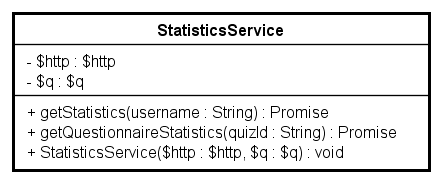
\includegraphics[scale=0.60]{UML/Classi/Front-End/QuizziPedia_Front-end_Services_StatisticsService.png}
	\caption{QuizziPedia::Front-End::Services::StatisticsService}
\end{figure}\FloatBarrier
\begin{itemize}
	\item \textbf{Descrizione}: questa classe permette di ottenere le statistiche dell'utente;
	\item \textbf{Utilizzo}: fornisce al controller le statistiche salvate;
	\item \textbf{Relazione con altre classi}:
	\begin{itemize}
		\item \textit{IN} \texttt{StatisticsController}: questa classe permette di le statistiche di un utente.
	\end{itemize}
	\item \textbf{Attributi:}
	\begin{itemize}
		\item \texttt{-} \texttt{\$http: \$http} \\ Campo dati che contiene un riferimento al servizio \$http che permette la comunicazione con il protocollo \textit{HTTP\ped{G}};
		\item \texttt{-} \texttt{\$q: \$q} \\ Campo dati che contiene un riferimento a \$q, un servizio offerto da \textit{AngularJS\ped{G}} per la gestione, tramite \textit{Promise\ped{G}}, di chiamate asincrone.
	\end{itemize}
	\item \textbf{Metodi:}
	\begin{itemize}
		\item \texttt{+} \texttt{StatisticsService(\$http: \$http, \$q: \$q)} \\ Metodo costruttore della classe \\
		\textbf{Parametri}:
		\begin{itemize}
			\item \texttt{-} \texttt{\$http: \$http} \\ Campo dati che contiene un riferimento al servizio \$http che permette la comunicazione con il protocollo \textit{HTTP\ped{G}};
			\item \texttt{-} \texttt{\$q: \$q} \\ Campo dati che contiene un riferimento a \$q, un servizio offerto da \textit{AngularJS\ped{G}} per la gestione, tramite \textit{Promise\ped{G}}, di chiamate asincrone.
		\end{itemize}
		\item \texttt{+} \texttt{getStatistics(username: String): Promise}: \\Metodo che serve per recuperare le statistiche di un utente tramite chiamata al back-end. Il metodo ritorna una \textit{Promise\ped{G}}. In caso la \textit{Promise\ped{G}} venga rifiutata, verrà restituito al \texttt{StatisticsController} un oggetto \texttt{ErrorModelInfo} contenente tutti i dettagli dell'errore. In caso la \textit{Promise\ped{G}} venga accettata, verrà restituito al chiamante del metodo il risultato della chiamata.\\
	    \textbf{Parametri}:
		\begin{itemize}
			\item \texttt{username: String} \\ Parametro che indica l'utente del quale andranno caricate tutte le statistiche.
		\end{itemize}
		\item \texttt{+} \texttt{getQuestionnaireStatistics(quizId: String): Promise} \\Metodo che restituisce le statistiche di un questionario.  Il metodo ritorna una \textit{Promise\ped{G}}. In caso la \textit{Promise\ped{G}} venga rifiutata, verrà restituito al \texttt{StatisticsController} un oggetto \texttt{ErrorModelInfo} contenente tutti i dettagli dell'errore. In caso la \textit{Promise\ped{G}} venga accettata, verrà restituito al chiamante del metodo il risultato della chiamata.\\
		\textbf{Parametri}:
		\begin{itemize}
			\item \texttt{quizId: String} \\ Parametro che indica il questionario del quale verranno caricate le statistiche.
		\end{itemize}
	\end{itemize}
\end{itemize}